\documentclass[12pt,letterpaper]{article}

\usepackage[utf8]{inputenc}			% Sets encoding to UTF-8
\usepackage{times}					% Use Times New Roman as the default font
\usepackage{setspace}				% Free document from ugly single spacing
\usepackage{graphicx}				% So image use is possible
\usepackage{enumerate}				% Allows use of specified list numbering (letters)
\usepackage{lastpage}				% Gives the last page number as an accessible number
\usepackage{fancyhdr}				% Makes "1 of 10" type page numbering possible
\usepackage[protrusion=true,
            expansion=true,
            final]{microtype}		% Improves hbox handling, reducing errors
\usepackage{url}					% Provides clickable URLs (in the bibilography)
\usepackage[sort&compress]{natbib}	% Need this for the bibliography to work properly
\usepackage[margin=1in]{geometry}	% Set margins to standard 1 inch margins
\usepackage{xurl}
\usepackage[breaklinks,
			colorlinks = true,
            linkcolor = blue,
            urlcolor  = blue,
            citecolor = blue,
            anchorcolor = blue]
            {hyperref}				% Makes TOC Links to content
%\usepackage{showframe}				% Uncomment for troubleshooting layout issues

% use the same font for URLs - better than courier...
\urlstyle{same}

% make the text easier to read
\onehalfspacing

% don't want page numbering until the abstract
\pagenumbering{gobble}

% setting up the "1 of 10" type page numbering
\pagestyle{fancy}

% remove the "fancy" header - too cluttered and not in original
\fancyhead{} %remove contents of header
\renewcommand{\headrulewidth}{0pt} % give header no space and thus remove horizontal line

% add the "1 of 10" type page numbering
\fancyfoot[C]{\begin{flushright}\begin{footnotesize}{\thepage} of \pageref{LastPage}\end{footnotesize}\end{flushright}}

% some aliases for organizations in the bibliography who need citations to show up in the references section
\defcitealias{Ocean2021}{Ocean Marketplace}
\defcitealias{Balancer2021}{Balancer Liquidity Bootstrapping Pools}

\begin{document}

\begin{titlepage}
\centering
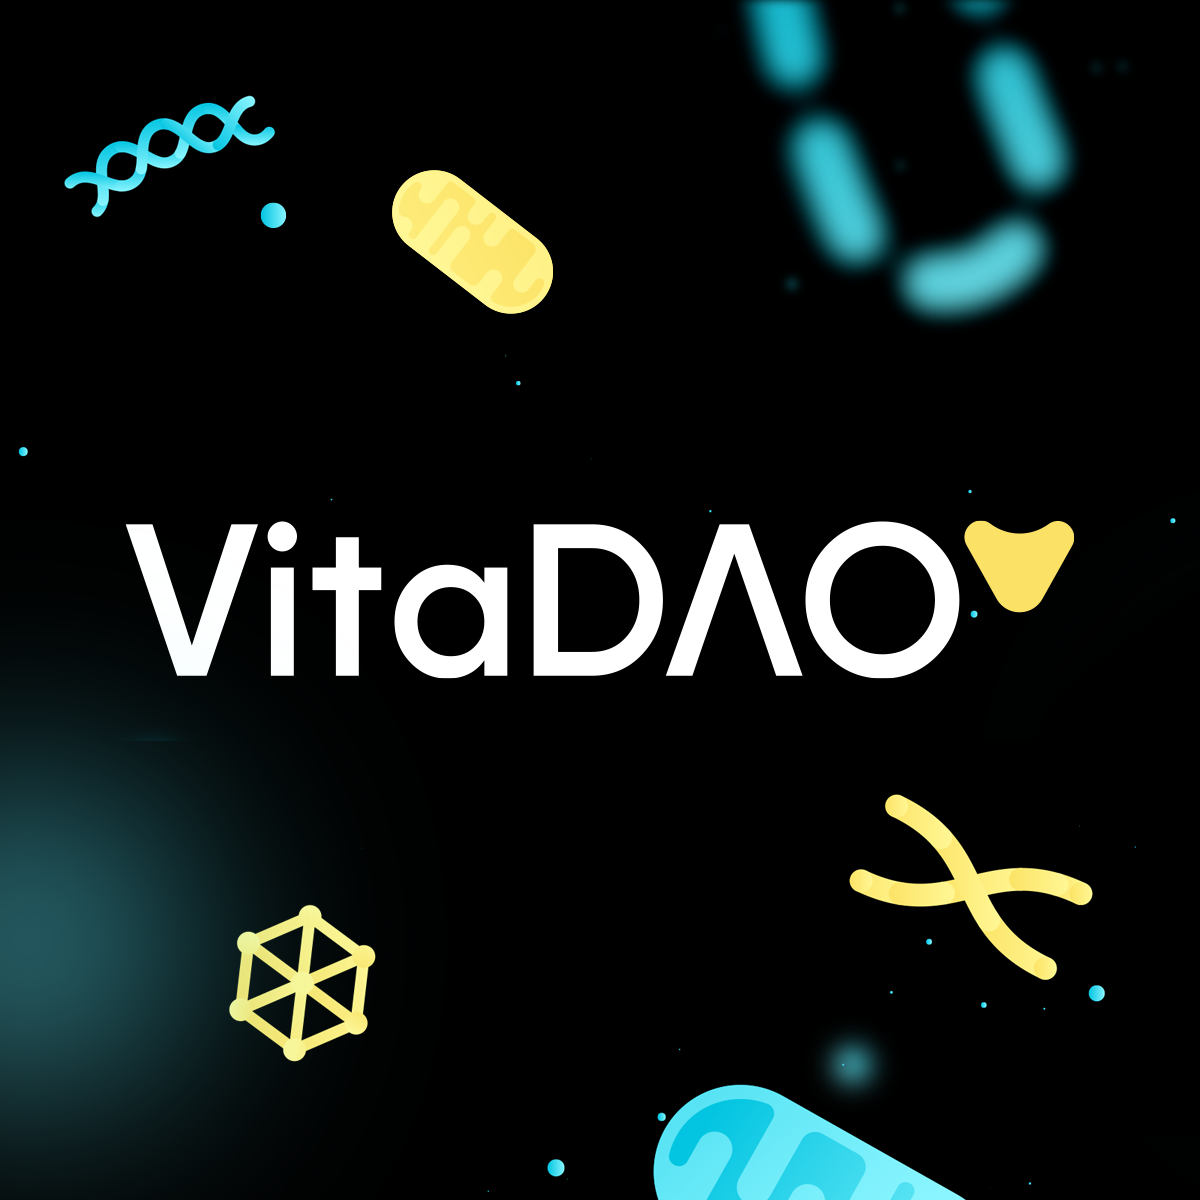
\includegraphics[width=\linewidth]{images/VitaDAO Opengraph.png} 
\\
\vspace{36pt}
{\begin{Large} \textbf{Whitepaper V0.1}\end{Large}}
\\
\vspace{18pt}
{\begin{large}{Authors: Tyler Golato, Paul Kohlhaas}\end{large}}
\\
\vspace{18pt}
{\begin{small}{Acknowledgments:  Jesse Hudson, Elad Verbin, James Brodie, Trent McConaghy, Robert Miller, Dimitri De Jonghe, Aubrey De Grey, Morten Scheibye-Knudsen, Theodor Walker}\end{small}}
\\
\vspace{18pt}
{\small\emph{(Draft open for public and community comment)}}
\end{titlepage}

\newpage

%start page numbering on the abstract page
\pagenumbering{arabic}

\begin{abstract}
% make the abstract section number be zero
\addtocounter{section}{0}
% add the abstract to the TOC, preserving section numbering
\addcontentsline{toc}{section}{\protect\numberline{\thesection}Abstract}

VitaDAO is a new cooperative vehicle for community-governed and decentralized drug development. Our core mission is the acceleration of R\&D in the extension of human life and health-span. Today, the biopharma industry booms with unprecedented late-stage investment, particularly in longevity science. However, the industry severely lacks critical \textit{early-stage} funding, and incentives between patients, researchers and industry are misaligned. To align incentives and vitalize early-stage funding in longevity biopharma, VitaDAO uses a combination of novel governance frameworks in decentralized autonomous organizations (DAOs), non-fungible tokens (NFTs), and financial engineering tools such as algorithmic automated market makers (AMMs), all of which run on the Ethereum blockchain.

At its core, biopharma value is intellectual property (IP) rights, domain specific know-how, and research data. Research and development is now prohibitively expensive and siloed, largely due to the way IP business models incentivize monopolization of innovation. This is done through the creation of patent thickets in protected portfolios. These IP mechanisms prevent open sharing of research data, inherently disincentivizing collaboration and transparency. They prevent the public and patients from having any real ownership in biopharma IP, despite their tax dollars funding most early-stage development. Outside of grants to fund basic research, early-stage funding for drug development is extremely limited. When drugs do finally make it to market, there exist strong incentives for price gouging.

VitaDAO solves some of these problems. An open cooperative anyone can join, VitaDAO’s goal is to support and finance new therapeutics and research data in longevity science. In exchange, VitaDAO will directly hold IP rights in the novel early-stage therapeutics it supports and funds. We will grow a portfolio of IP and data assets, which we can make available and monetize through novel data marketplaces such as \citetalias{Ocean2021}. This promotes both open science and new business models.

Ownership of VitaDAO and its governance require VITA tokens. To obtain VITA tokens, a person or organization can contribute work, funds, or other resources like data and IP to VitaDAO. Ownership of VITA allows the holder to participate in democratic governance of VitaDAO, and thus direct its research, access and monetize its data repositories, and manage its IP portfolio.

\end{abstract}

\newpage
% Make it read "Table of Contents" and center
\renewcommand{\contentsname}{\centering Table of Contents}

% Keep the TOC simple
\tableofcontents

\newpage

\section{Introduction}
Current biopharma business models carry severe limitations and R\&D inefficiencies at the cost of those who should be the core stakeholders: the patients in need of medication and researchers discovering new therapeutics.

\subsection{Intellectual Property in Biopharma}
Fundamentally, value creation in biopharma requires building two core assets: intellectual property (IP) and research and development (R\&D) data \citep{Chandra2011}. When companies explore a use case for a new therapeutic, they patent their discoveries to gain IP. IP enables them to secure future revenue and recoup the high costs of R\&D. As companies invest billions of dollars into generating data to bring therapeutics to market, they offset this by selling equity ownership or IP royalty rights in the form of future drug sales or milestone based payments. \citep{Wouters2020}. While IP in theory incentivizes innovation, in practice it does the opposite. IP ownership as a business model barely evolved in the past century, remaining mainly extensive legal contracts and bureaucratic complexities. IP is one of the most valuable asset classes in the world but it remains rigid, largely illiquid, and difficult to transfer.

IP owners and sellers who seek to monopolize commercial value have incentives to withhold negative research data. This creates a principal-agent dilemma and, in part, leads to a phenomenon coined the “reproducibility crisis” \citep{Sherkow2017}. Pharma tends to only share positive R\&D data which leads companies to waste enormous resources repeating each others’ failures because without complete data, clinical and preclinical studies are often not reproducible. 

The current system severely lacks incentives for open science, collaboration, and data sharing \citep{Ali-Khan2017}. IP Owners downplay side effects or indicators of lower effectiveness in favor of profit maximization. Valuable research findings are lost for the broader scientific community and not considered during patient treatment. Monopolistic IP ownership within biopharma companies leads to centralization, and the disincentivization of collaboration. Promising drug candidates often fall to the wayside for organizational, political, or competitive reasons. These centralized and siloed research efforts lead to the high R\&D cost and long time-to-market plaguing pharma today. The excess cost ranges from \$800 million to \$2.6 billion on average in cost, and time to market takes upwards of 10 years \citep{DiMasi2016}. On a macro scale, this IP model leads to incentive misalignment and information asymmetry. 

Lastly, the current financing and investment landscape restricts access and participation to early-stage biopharma from its most important stakeholders: patients and researchers. In the US, generally only accredited investors can finance early-stage ventures \citep{Rowley2018}. The market is opaque, and no singular or efficient marketplace exists to discover or access these opportunities in a transparent fashion.

We need more democratic, open, and transparent models. Collaboration and open research in the scientific community could bring down the rising cost of drug development \citep{Bookbinder2020}.

\subsection{The Evolution of Pharma and the Valley of Death}
There is a significant shift underway in the pharmaceutical industry's process of drug development. Increasingly, smaller biotech firms leverage recent academic research in the life sciences to develop new drugs, and then pharmaceutical giants acquire these smaller firms and their expertise using their access to low-cost capital \citep{Huang2021} Notably, much of the funding for this academic work comes from grants or public capital, but  pharmaceutical companies then privatize it so the public receives little upside from the research it funded \citep{Toole2004}. The number of biotech startup companies formed due to technology licensing increased dramatically in recent years, from 145 in 1994 to 278 in 2000 to 1,024 in 2016. The increase is on an exponential curve. Of the 30 top-selling drugs worldwide in 2000, only five traced back to universities and the remaining 25 were developed by big pharma. By 2018 however, more than half of the top 30 drugs were sourced from academia \citep{Huang2021}. Biotech universities increasingly prove themselves as untapped goldmines of valuable IP, yet often these assets are unavailable for investment until a startup spins up. 

Assets from universities not out-licensed or spun out into startups remain in a difficult limbo, known as "The Valley of Death," where they often fail to move forward \citep{Seyhan2019}. Many of these technologies have extreme value to patients, but because of this system, they never ultimately serve the populations intended to benefit from them. These assets require investment and capital injections at a much earlier stage. The market desperately needs new open commercialization models to incentivize their development. We need a creator economy for researchers and universities, as they are one of humanities greatest assets. 

\subsection{Longevity Will Transform Our Approach To Medicine}
Longevity science has the power to completely transform global healthcare. Age-related diseases are among the most significant contributors to our global health burden and are responsible for the highest costs incurred by healthcare systems \citep{WHO2011}. 

The longevity space is experiencing a tremendous boom, in part because of its ability to address this problem. The space is evolving rapidly in terms of understanding the aging process and its capacity to develop health and life-extending therapeutics \citep{ARDD2020}. It is now a routine procedure to reverse the aging of human cells in the laboratory. Correspondingly, the economics of investing in longevity are more attractive than ever. There are 100s of new companies and funds dedicated to research and product development in the fields of senolytics, telomeres, stem cells, mitochondria, and gene editing \citep{Pfleger2021}. These are some of the core domains from which therapies that increase lifespan will emerge. However, aging is not recognized as a disease, and this has created barriers to prescribing drugs for aging itself \citep{Suresh2014}. 

The rush of investment into the field has the potential to rapidly accelerate these developments but also comes with distinct problems. The centralization of aging research by large institutions and billionaires has the potential to create the same problems and pitfalls that plague the pharmaceutical industry: lack of transparency, restricted access, and concentrated control over therapeutics that should be made widely available to anyone at an affordable price. 

We believe the future of health and life-extension should be open, collaborative, and community-owned. We see longevity as an entirely new approach to medicine, one that has the potential to prevent, as opposed to treat or intervene. This approach will completely change the way the world provides medical care and will profoundly impact society.

\section{Solution}
\textbf{We propose the creation of VitaDAO: the first fully open, community-owned, and transparent longevity intellectual property collective.}

Members of the public can become co-owners of VitaDAO and its IP by purchasing VITA via contributing funds, valuable research data, IP assets, or services to VitaDAO. VITA tokens grant Ownership and governance of VitaDAO. Ownership of VITA allows the holder to participate in the democratic governance of VitaDAO, and thus direct its research, access and monetize its data repositories, and manage its IP portfolio.

VitaDAO will acquire IP rights and R\&D data, and also commission research to further develop its assets. VitaDAO's core assets will consist of:
\begin{enumerate}
\item IP, including patents and licenses to therapeutics.
\item R\&D data assets generated by funding research projects.
\item Funds stored in its treasury, including unissued VITA.
\end{enumerate}

To acquire and finance specific research proposals, VitaDAO members may elect to issue tokens. VitaDAO can do this on a continuous or per-project basis, using automatic market makers (AMMs) like \citetalias{Balancer2021} (LBPs) that enable a fair and transparent participation for prospective members. 

In order to monetize and manage IP and data assets, VitaDAO members may elect to attach them to Non-Fungible Tokens (NFTs) as detailed below in Section 4.

\subsection{Stakeholders}
VitaDAO will rely on service providers (initially its advisers, Molecule, and other web3 development teams) to facilitate various administrative and developmental functions. Work done by these providers will include the purchase and transfer of IP from universities, updating and maintaining the dapp, validating and formatting information selected by members, and handling other interactions that may emerge over its initial genesis and lifecycle.

\vspace{15pt}
\begin{center}
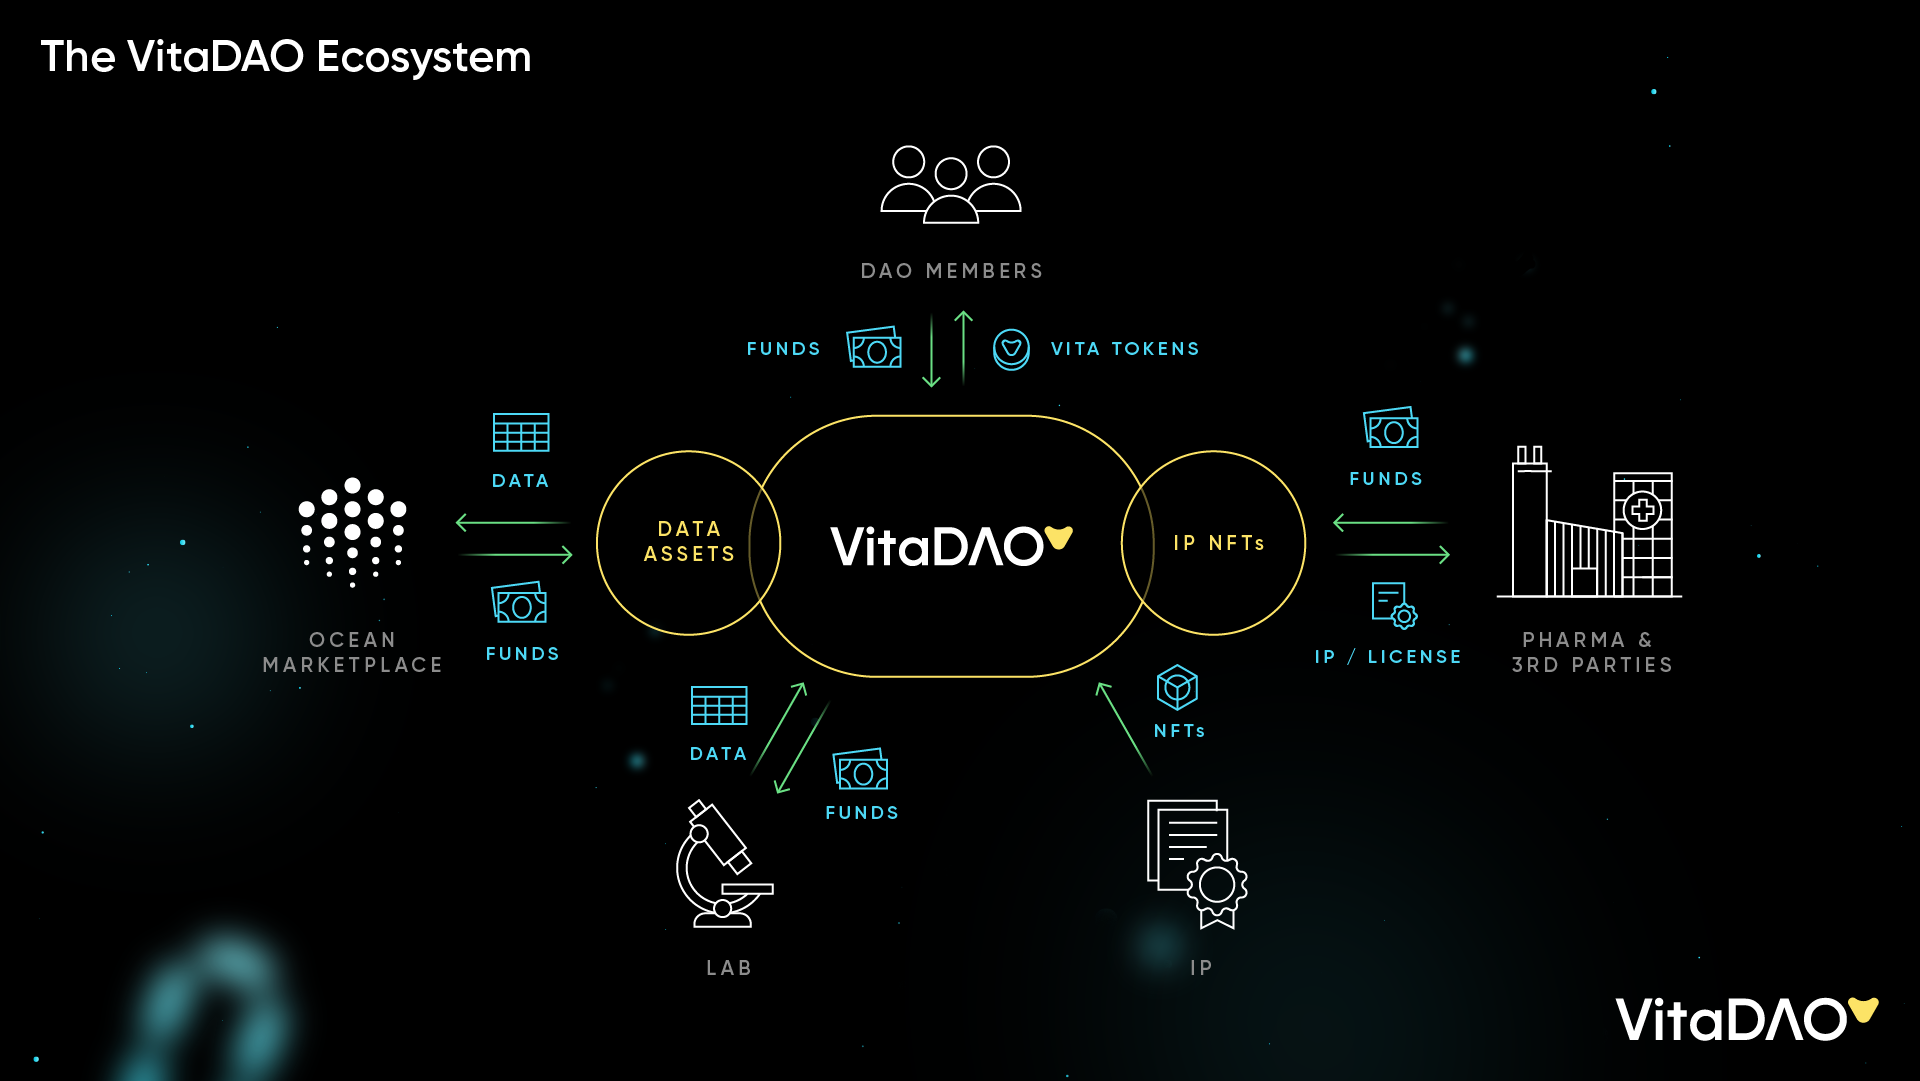
\includegraphics[width=\linewidth]{images/VitaDAO Diagram - Ecosystem-p-1600.png} 
\end{center}

\section{Core Architecture}

\subsection{Organization and Governance}
VitaDAO is an unincorporated association consisting of several core components including:
\begin{enumerate}
\item VitaDAO’s governance smart contracts, modeled after Moloch DAO and the LAO.
\item VitaDAO’s contribution and liquidity bootstrapping mechanism utilizing Balancer LBPs.
\item VitaDAO’s IP and data assets, which are represented as NFTs.
\end{enumerate}
VitaDAO’s smart contract architecture enables members who own VITA to freely engage in governance decisions pertaining to the assets and funds held by VitaDAO. Members will manage VitaDAO with a dapp, through which they will interact with VitaDAO’s smart contracts and facilitate the purchase, funding, and management of IP and data assets.

VitaDAO members will not only govern the existing structure but also vote on how to refine its structure and governance processes. Because VitaDAO members fully control the governance of VitaDAO, they not only vote, but also make proposals on which to vote. Proposals come in several types: governance proposals, project proposals, funding proposals, data monetization proposals, and IP proposals. As needed, VitaDAO can add or modify proposal types and their governance.

To provide the level of industry expertise required to effectively and thoroughly evaluate therapeutics projects, VitaDAO will elect a council of 3-6 industry experts to review its projects, data and IP. This council assists in submitting proposals to the VitaDAO members.

The initial goal of VitaDAO is to mimic successful execution patterns in the biotech industry, while improving or replacing those that do not work well. Over time, we expect further governance mechanisms to emerge around VitaDAO.

In summary:
\begin{enumerate}
\item VitaDAO members are in full control of the governance of VitaDAO via votes and proposals.
\item VitaDAO will elect a council of industry experts to review its projects, data and IP. 
\item VitaDAO may engage service providers spanning patent attorneys, contract research firms or third party experts.
\item VitaDAO’s initial goal is to mimic successful execution patterns in the biotech industry.
\end{enumerate}

\subsection{"Genesis Bootstrapping and Liquidity"}
For its initial genesis, VitaDAO will deploy a Balancer LBP to enable interested participants to contribute funds to its treasury and join the collective. As VitaDAO grows, members may elect to create additional LBPs to on-board further projects.

We anticipate the initial genesis will operate as follows:
\begin{enumerate}
\item VitaDAO will allocate a small amount of its fixed token supply into a Balancer LBP with the goal to raise sufficient funds to finance the first research project for two years. The community will decide on the full fundraising budget and structure pending simulations and crypto economic modeling using cadCAD.
\item The LBP allows the community to contribute funds and join VitaDAO for the first time. Simultaneously, the pool acts as an important first price discovery mechanism. Individuals wishing to join may contribute a multitude of assets, such as ETH, USDC or Ocean and receive VITA tokens according to the corresponding dollar value. The primary currency of the LBP will be USDC to ensure price stability.
\item After a fixed period, the LBP resolves, forwarding its acquired funds to VitaDAO and kick-starting its operation. Should the LBP fail to reach a specific threshold participants may withdraw their stakes.
\end{enumerate}

\section{Holding and Managing IP and Data Assets as NFTs}

\subsection{Intellectual Property Rights}
VitaDAO will directly hold IP rights in underlying research projects and will develop a growing portfolio of assets represented as NFTs using the  novel IP NFT framework developed by Molecule. Molecule’s IP NFT system allows the holder of an existing piece of IP (in the form of a license or patent) to attach it to an NFT and transfer it to a new owner.

Upon IP NFT creation, the creator must sign a cryptographic message that prints their signature onto an IP licensing agreement. When the NFT changes owners, the transaction requires both buyer and seller of the NFT to sign a message that references the IP license agreement, which includes references to the transaction, the buyer and seller’s respective identities, and legal signatures modeled after the legal Signature Algorithm pioneered by \citet{OpenLaw2019}.

%ADD SECTION ON NFT fractionalisation, sharding, royalty streams. 
%https://tokeneconomy.co/token-bonding-curves-in-practice-3eb904720cb8

Initially, VitaDAO will hold IP in research projects for longevity therapeutics in the form of licenses. These licenses enable VitaDAO or its designated service providers to file for patents, monetize the IP, and contract researchers to grow the value of the underlying assets.

\subsection{Data Assets}
Besides owning IP rights related to individual projects, VitaDAO will also own data assets and research outputs from the R\&D it funds. VitaDAO will hold custody over these assets, while making them available to its members and others, and monetizing them via data marketplaces such as Ocean Marketplace. VitaDAO may attach these data assets to NFTs where useful and applicable. 

VitaDAO’s introduction of its data assets into Web3 will drive fluid price discovery and liquidity for each individual data set as buyers and sellers engage with them and curate the most valuable findings. Obfuscation of data assets and enabling secure computation on them will be a highly relevant future use case that Web3 protocols such as Ocean Protocol could facilitate. The applications around composability and interoperability here are manifold, and once VitaDAO is live those applications will receive further exploration.

Data assets could include, but are not limited to: laboratory updates and reports, processed data, quarterly updates, western blot data, qPCR data, cell culture experiments, survival analysis, sequence data, western blot gels, microscopy and cell culture. These data assets could be in the forms of raw data, images or PDFs.

The type of data assets and their monetization potential are summarized below:
\begin{enumerate}
\item \textbf{Public Data Assets:} All data in these assets are view-able by members, who can vote to list these data packages on Ocean Marketplace.
% NEXT ITEM NEEDS SOURCE
\item \textbf{IP Data Assets:} Required for filing of patents or further IP. These assets will be obfuscated as they could compromise filing of IP. These assets could end up on Ocean Marketplace after they have IP filed to protect them.
\item \textbf{Progress Data Assets:} Intended to keep DAO members up-to-date on ongoing research findings and serving as proof of progress. This data has a certain level of obfuscation, meaning any information capable of compromising the intellectual property itself will be hidden. Such data would not be relevant for Ocean Marketplace.
\end{enumerate}
Members wishing to engage with the IP, review the data assets directly, or engage with the council may need to submit KYC documentation and sign non-compete and confidentiality agreements to help ensure the viability of the assets for all members.

\section{Staking and Signaling}
Members can use VITA tokens to signal long-term support for individual projects. A member may stake their VITA tokens for a set time period until a project milestone is reached (e.g. 3 months/6 months/12 months). Projects predetermine milestones and they must be measurable. Their outcome is uncertain, however, meaning members take additional risk by foregoing liquidity.

When a project reaches a milestone, staked tokens unlock. In return for locking tokens, VitaDAO pays out regular signaling rewards to stakers. This process sends valuable signals to the market, as it showcases the confidence of members in specific projects. Furthermore, it reduces volatility and creates a circular economy to members, who actively contribute value and review project success.

We anticipate implementing signaling after the first successful project runs an initial funding cycle, giving members time to sufficiently model this mechanism and implement it in VitaDAO V2.

\section{Genesis \& First Project Lifecycle}
The following section details the initial Genesis project acquisition and models out a potential first project lifecycle. After Genesis and instantiation of its governance mechanism, VitaDAO members will vote to incorporate the first longevity therapeutic into its collective by purchasing an NFT attached to IP of a longevity project from the Scheibye-Knudsen Laboratory at the University of Copenhagen. Once the acquisition is complete, members can vote to allocate a first tranche of funding to the University of Copenhagen to commence research.

The project lifecycle could operate as follows:
\begin{enumerate}
\item VitaDAO proposes to purchase the Scheibye-Knudsen Laboratory IP NFT.
\item VitaDAO members vote on the proposal and define the project parameters and payment schedules with the Scheibye-Knudsen Laboratory.
\item The project commences as VitaDAO completes a first payment to initiate the preclinical studies.
\item The Scheibye-Knudsen Laboratory begins delivering first data assets consisting of progress reports, raw data and initial findings.
\item First definitive findings are in, and VitaDAO members, supported by industry advisers, decide how to use the data and further commercialize the asset. This could result in:
\begin{enumerate}[a.]
\item Filing for further IP and patents.
\item Filing for clinical trials and further studies.
\item Monetizing the data sets through Ocean Marketplace.
\end{enumerate}
\item Simultaneously, VitaDAO may decide to launch further LBPs for additional projects at any point, which are sourced through its community, or to raise additional funding for the Scheibye-Knudsen Laboratory.
\end{enumerate}

\section{Exit Scenarios and IP Commercialization}
If the research data surrounding an asset is sufficiently positive and clinical trials are attractive, VitaDAO can license or sell its IP or data to institutional stakeholders, such as pharmaceutical or biotech companies. Given enough liquidity and governance sophistication, VitaDAO could even attempt to bring these assets to market itself. Members of VitaDAO will decide on how to distribute income generated from successful IP monetization.

Individual IP and NFTs may be spun out into separate fractionalized markets to enable more granular participation by the public. From a technical perspective, this would entail moving the NFT and associated data sets out of custodianship of VitaDAO and into a sub-DAO represented by a new ERC20 token. Members of VitaDAO may elect to spin out a project to:
\begin{enumerate}
\item Enable the project and IP to raise additional funding from a wider community.
\item Create exit scenarios for VitaDAO and further decentralize project ownership.
\item Enable more granular fundability and participation on a project level.
\end{enumerate}

\section{Open Research Questions}
The mechanics described in this paper are novel, experimental, and rely on multiple moving parts, especially the creation of an active tokenized governance community. Our goal is to tackle these questions together as a community and through multiple working groups that include industry experts, as these experts will substantially improve the system’s long-term potential.
\begin{enumerate}
\item \textbf{Governance and effective collective decision-making on drug development projects:} can a decentralized community effectively govern and attract the expertise required to successfully commercialize therapeutics? Will the token-based voting mechanism described herein succeed in generating positive outcomes?
\item \textbf{Biopharma business logic:} will the biopharma industry be open to purchasing IP and patents produced by a decentralized collective, as opposed to current business practices? Will VitaDAO be able to support a sufficient number of projects to become positive-sum at scale?
\item \textbf{Legal and patent law:} can VitaDAO successfully file for further patents on the IP assets it manages or will it have to rely on third parties? In case of patent litigation against VitaDAO, is it able to protect the validity of the IP as a normal company could?
\end{enumerate}

\section{Conclusion}
The open IP and data ownership structures presented here could help alleviate some of the most severe challenges in the current pharmaceutical and biotech pipeline, and could help create a future of open and democratic ownership of longevity therapeutics. 

IP collectives like VitaDAO can help realign incentives with neglected stakeholder groups - patients and scientists - by creating alternative democratic research structures that distribute value and governance more evenly. Imagine research on a new breakthrough insulin treatment funded by diabetics who believe in it and stand to benefit the most from it. What would this do to access and pricing?

Separating R\&D data creation from IP ownership helps overcome a costly principal-agent dilemma and the current reproducibility crisis. In an openly traded curation market and structure, both negative and positive data might surface much sooner and allow the best therapeutics to succeed. Transparent financialization of data  and open composability with decentralized financial markets opens up entirely new and accelerated funding models to promising scientists and laboratories across the globe. 

From an industry perspective, we believe IP cooperatives like VitaDAO will be a win-win situation for all stakeholders: biopharma, researchers, and patients. It combines traditional industry IP holding structures with novel, tokenized ownership accessible by anyone wishing to contribute to the research. In doing so, it drives valuable innovation in the biopharma industry.

% Need to clear page so reference page doesn't get messed up from above
\clearpage

% Make references show up in the TOC
\addcontentsline{toc}{section}{References} 

% fix inevitable underfull and overfull hboxes due to including urls in the reference section
% this is a suboptimal fix due to a url that uses 7 query string parameters, it beat me down
\raggedright 

% Add APA style Bibliography
\bibliography{references}
\bibliographystyle{apalike} 


\end{document}